\selectlanguage{italian}

\section{Radioattività}

I primi indizi verso la radioattività sono derivati dalla rilevazione dei raggi X: questi sono onde elettromagnetiche, ovvero fotoni, generate da transizioni di elettroni tra livelli energetici ($ \Delta E_e = \hbar \omega $); questi dunque non sono processi nucleari, dato che avvengono all'interno della nube elettronica dell'atomo.\\
Quando si parla di radioattività in senso stretto, però, si fa riferimento ai decadimenti dei nuclidi.

\subsection{Decadimenti radioattivi}

I decadimenti radioattivi sono processi in cui un nuclide stabile raggiunge una configurazione con energia più bassa emettendo spontaneamente radiazione.\\
Utilizzando un campo magnetico, Rutherford riuscì a distinguere tre tipologie di radiazione, e dunque di decadimenti radioattivi:
\begin{enumerate}
  \item decadimento $ \alpha $, in cui la radiazione è costituita da un nucleo di $ \ch{^4_2 He} $ ed è poco penetrante, coinvolge l'interazione elettromagnetica e quella forte;
  \item decadimento $ \beta^{\pm} $, in cui la radiazione è costituita da un $ e^{\pm} $ ed è mediamente penetrante, coinvolge l'interazione debole:
    \begin{itemize}
      \item decadimento $ \beta^- $: $ n \rightarrow p^+ + e^- + \bar{\nu}_e $;
      \item decadimento $ \beta^+ $: $ p^+ \rightarrow n + e^+ + \nu_e $;
    \end{itemize}
  \item decadimento $ \gamma $, in cui la radiazione è costituita da un fotone con energia dell'ordine delle decine di MeV, dunque estremamente penetrante.
\end{enumerate}
A questi si aggiunge la cattura elettronica, un decadimento in cui un nuclide proton-rich cattura un elettrone dalle shell interne dell'atomo, seguendo la reazione $ p^+ + e^- \rightarrow n + \nu_e $, emettendo raggi X a seguito del rimpiazzo dell'elettrone interno con uno dalle shell esterne.

\subsection{Energy balance}

Un decadimento radioattivo può essere visto come un caso particolare di reazione nucleare; è quindi possibile definire il $ Q $-value del decadimento come la differenza di energia a riposo (massa) tra reagenti (nuclide instabile) e prodotti, così da poter stabilire qualora esso sia possibile, ovvero spontaneo, con la condizione $ Q > 0 $.\\
In particolare, si definiscono i $ Q $-values dei seguenti decadimenti:
\begin{enumerate}
  \item decadimento $ \alpha $: $ Q_{\alpha} \equiv \left[ M(Z,A) - M(Z-2,A-4) - m(\ch{^4_2 He}) \right] c^2 $;
  \item decadimento $ \beta^- $: $ Q_{\beta^-} \equiv \left[ M(Z,A) - M(Z+1,A) - m_e \right] c^2 $;
  \item decadimento $ \beta^+ $: $ Q_{\beta^+} \equiv \left[ M(Z,A) - M(Z-1,A) - m_e \right] c^2 $;
  \item electron capture: $ Q_{e} \equiv \left[ M(Z,A) + m_e - M(Z-1,A) \right] c^2 $;
\end{enumerate}
Si vede subito che $ Q_e > Q_{\beta^+} $: di conseguenza, nell'electron capture i prodotti di decadimento hanno maggior energia cinetica disponibile, inoltre ci sono dei casi in cui può avvenire l'electron capture ma non il decadimento $ \beta^+ $.

\subsection{Radioactive decay law}

Il processo di decadimento ha natura aleatoria, dunque va trattato in maniera statistica.\\
Il numero di decadimenti al secondo è proporzionale al numero di nuclidi radioattivi:
\begin{equation}
	- \frac{dN}{dt} = \lambda N(t)
	\label{eq:2.1}
\end{equation}
Si trova quindi la legge di decadimento esponenziale:
\begin{equation}
	N(t) = N_0 e^{-\lambda t}
	\label{eq:2.2}
\end{equation}
Si definisce inoltre il decay rate (o activity) come $ A(t) \defeq \lambda N(t) $, misurato in Bequerel $ 1\,\text{Bq} = 1 \,\text{decay}/\text{s} $ o in Curie $ 1\,\text{Ci} = 3.7\cdot10^{10}\,\text{Bq} $ (activity di $ 1\,\text{g} $ di radio). Si definiscono inoltre la half-life $ t_{1/2} \equiv \frac{\ln 2}{\lambda} $ e la vita media $ \tau = \frac{1}{\lambda} $ rispettivamente come il tempo dopo il quale il campione si è ridotto di $ \frac{1}{2} $ e di $ \frac{1}{e} $: si ha $ t_{1/2} \approx 0.693 \tau < \tau $.\\
Per i decay rates si trova facilmente che, definendo $ A_0 \equiv \lambda N_0 $:
\begin{equation}
	A((n+1)t) = A(t) \left( \frac{A(t)}{A_0} \right)^n
	\label{eq:2.3}
\end{equation}
Nel caso di una miscela di radioisotopi, è possibile risalire alle singole costanti di decadimento nel caso in cui le vite medie siano molto diverse, poiché quando la specie con la $ \tau $ più corta è completamente decaduta si può misurare direttamente la $ \lambda $ dell'altra specie, per poi risalire a quella della prima tramite la differenza delle activities.

\subsubsection{Decay branches}

Può capitare che lo stesso nuclide radioattivo possa decadere in due o più modi differenti, detti decay branches: detta $ \lambda_k $ la costante di decadimento parziale della $ k $-esima branch, nel caso di $ n $ branches si ha:
\begin{equation}
	\lambda \equiv \lambda_1 + \dots + \lambda_n
	\label{eq:2.4}
\end{equation}
e questa costante totale è l'unica che si osserva, anche quando si rileva una sola delle branches. Si definiscono i branching ratios come $ B_k \defeq \frac{\lambda_k}{\lambda} $.

\subsubsection{Decay chains}

Spesso, in un decadimento radioattivo, capita che anche i prodotti siano radiaottivi: ciò dà vita ad una catena di decadimenti $ N_1 \xrightarrow{\lambda_1} N_2 \xrightarrow{\lambda_2} N_3 \dots $, dove le $ \lambda_k $ sono diverse tra loro.\\
Una decay chain è descritto da un sistema di coupled differential equations. Nel caso, ad esempio, di un doppio decadimento (quindi con prodotto $ N_3 $ stabile):
\begin{equation}
	\begin{cases}
		\dot{N}_1 = - \lambda_1 N_1 \\
		\dot{N}_2 = \lambda_1 N_1 - \lambda_2 N_2 \\
		\dot{N}_3 = \lambda_2 N_2
	\end{cases}
	\quad\Longrightarrow\quad
	\begin{cases}
		N_1(t) = N_0 e^{-\lambda_1 t} \\
		N_2(t) = \frac{\lambda_1}{\lambda_1 + \lambda_2} N_0 \left( e^{-\lambda_1 t} - e^{-\lambda_2 t} \right) \\
		N_3(t) = \frac{\lambda_1 \lambda_2}{\lambda_1 + \lambda_2} N_0 \left( \frac{1 - e^{-\lambda_1 t}}{\lambda_1} - \frac{1 - e^{-\lambda_2 t}}{\lambda_2} \right)
	\end{cases}
	\label{eq:2.5}
\end{equation}
La soluzione generale al caso di $ n $ decadimenti è dato dall'\textit{equazione di Bateman}:
\begin{equation}
	N_k(t) = \sum_{i = 1}^{k} \left[ N_0^{(i)} \left( \prod_{j = 1}^{k-1} \lambda_j \right) \left( \sum_{j = i}^{k} \frac{e^{-\lambda_j t}}{\prod_{p=i, p\neq j}^{k} (\lambda_p - \lambda_j)} \right) \right]
	\label{eq:2.6}
\end{equation}

\paragraph{Equilibrio radioattivo} Si parla di equilibrio radioattivo quando la specie radioattiva madre e quella figlia hanno la stessa attività, ovverosia quando la specie figlia decade allo stesso rate a cui è prodotta. In una decay chain, l'equilibrio radioattivo può instaurarsi tra ciascuna coppia di nuclidi della catena: la condizione generale da soddisfarre è che $ (t_{1/2})_{\text{madre}} > (t_{1/2})_{\text{figlia}} $.\\
In particolare, si parla di:
\begin{enumerate}
	\item equilibrio transiente: si ha quando $ (t_{1/2})_{\text{madre}} \approx (t_{1/2})_{\text{figlia}} $, dunque, dopo un periodo di transienza iniziale, l'activity della specie madre e quella della specie figlia diventano uguali;
	\item equilibrio secolare: si ha quando $ (t_{1/2})_{\text{madre}} \rightarrow \infty $ (comparabile all'età della Terra), dunque la sua activity è praticamente costante; di conseguenza, dopo un certo periodo di tempo, anche l'activity della specie figlia diventerà costante e pari a quella della specie madre (si vede analiticamente dall'Eq. 2.5 ponendo $ \lambda_1 \ll \lambda_2 $). Si parla di equilibrio secolare anche quando, più genericamente, $ (t_{1/2})_{\text{madre}} \gg (t_{1/2})_{\text{figlia}} $.
\end{enumerate}

\paragraph{Serie radioattive naturali}

Ci sono 4 serie decay chains naturali principali, tutte composte da decadimenti $ \alpha $ e $ \beta^- $:
\begin{enumerate}
  \item serie del torio: inizia col $ \ch{^{232} Th} $ e termina col $ \ch{^{208} Pb} $, il decadimento col tempo di dimezzamento più lungo è $ \ch{^{232} Th} \rightarrow \ch{^{228} Ra} $ con $ t_{1/2} = 14 \,\text{Gy} $;
  \item serie dell'uranio: inizia col $ \ch{^{238} U} $ e termina col $ \ch{^{206} Pb} $, il decadimento col tempo di dimezzamento più lungo è $ \ch{^{238} U} \rightarrow \ch{^{234} Th} $ con $ t_{1/2} = 4.5 \,\text{Gy} $;
  \item serie del plutonio: inizia col $ \ch{^{239} Pu} $ e termina col $ \ch{^{207} Pb} $, il decadimento col tempo di dimezzamento più lungo è $ \ch{^{235} U} \rightarrow \ch{^{231} Th} $ con $ t_{1/2} = 0.71 \,\text{Gy} $;
  \item serie del nettunio: inizia col $ \ch{^{237} Np} $ e termina col $ \ch{^{209} Bi} $, il decadimento col tempo di dimezzamento più lungo è $ \ch{^{237} Np} \rightarrow \ch{^{233} Pa} $ con $ t_{1/2} = 2.3 \,\text{My} $;
\end{enumerate}
Quest'ultima serie non è più osservabile in natura poiché la sua vita media non è comparabile con l'età della Terra, a differenza delle altre tre.

\paragraph{Carbon dating}

Il $ \ch{^{14}C} $ è un isotopo radioattivo del carbonio con $ t_{1/2} = 5730\,\text{y} $; nonostante questa vita media relativamente corta, esso è prodotto continuamente grazie ai raggi cosmici in atmosfera tramite neutron capture: $ \ch{^{14}N} + n \rightarrow \ch{^{14}C} + p^+ $; una volta assorbito dai sistemi biologici, esso decade per decadimento $ \beta^- $: $ \ch{^{14}C} \rightarrow \ch{^{14}N} + e^- + \bar{\nu}_e $.\\
Misurata la specific activity $ a $ del campione da datare, si può risalire al time since death comparandola alla standard specific activity $ a_0 = 0.266\,\text{Bq}/\text{g} $: $ T = \frac{t_{1/2}}{\ln 2} \ln \frac{a}{a_0} = - 8033\,\text{y} \cdot \ln \frac{a}{a_0} $.\\
L'assunzione fondamentale di questo metodo di datazione è che la concentrazione naturale di $ \ch{^{14}C} $ rimanga costante nel tempo: con la Guerra Fredda questo è diventato un problema, poiché i test nucleari hanno fatto raddoppiare per un periodo tale concentrazione, e solo ultimamente si sta tornando ai livelli precedenti. Inoltre, va notato che il carbon dating è efficacie solo per oggetti non più vecchi di 50'000 anni: per epoche precedenti, sono necessari altre coppie isotopiche, come ad esempio $ \ch{^{40}K} $ - $ \ch{^{40}Ar} $, $ \ch{^{235}U} $ - $ \ch{^{207}Pb} $ o $ \ch{^{238}U} $ - $ \ch{^{208}Pb} $.

\section{Decadimento \texorpdfstring{$ \alpha $}{TEXT}}

Il decadimento $ \alpha $ consiste nell'emissione di un nucleo di $ \ch{^4 He} $ da parte di un nucleo instabile, secondo la reazione:
\begin{equation}
	\ch{^A_Z X_N} \rightarrow \ch{^{A-4}_{Z-2} Y_{N-2}} + \ch{^4_2 He_{2}}
	\label{eq:2.7}
\end{equation}
Questo avviene grazie alla repulsione coulombiana tra nucleo e $ \alpha $, espressa dall'andamento dell'energia potenziale:
\begin{equation}
	U(r) = \frac{2(Z-2)e^2}{4\pi \epsilon_0 r}
	\label{eq:2.8}
\end{equation}
È il decadimento prevalente nei nuclei pesanti: ad elevati $ A $ conviene ridurre la massa del sistema per acquisire maggiore stabilità (si veda Fig. \ref{bind-en}). Per lo stesso motivo, non si osservano decadimenti $ \alpha $ in nuclei più leggeri del $ \ch{^{126}_{62} Sm} $.

\paragraph{Bilancio energetico}

È fondamentale studiare il bilancio energetico del decadimento $ \alpha $: in particolare, esso è possibile quando il $ Q $-value dell'Eq. $ \ref{eq:2.7} $ è positivo. Assumendo che il nuclide instabile sia inizialmente a riposo:
\begin{equation}
	Q = T_{\ch{Y}} + T_{\alpha} = \left( m_{\ch{X}} - m_{\ch{Y}} - m_{\alpha} \right) c^2
	\label{eq:2.9}
\end{equation}
A ciò va aggiunta la conservazione del momento lineare, la quale impone che $ \ve{p}_{\ch{Y}} = -\ve{p}_{\alpha} $, con la quale si trova (trattando non-relativisticamente, dato che i valori tipici sono $ T_{\alpha} \sim 5\mev $):
\begin{equation}
	T_{\alpha} = \frac{m_{\ch{Y}}}{m_{\ch{Y}} + m_{\alpha}} Q \approx \left( 1 - \frac{4}{A} \right) Q
	\label{eq:2.10}
\end{equation}
Dunque $ \alpha $ trasporta circa il $ 98\% $ del $ Q $-value ($ \sim 5\mev $), mentre il restante $ 2\% $ ($ \sim 0.1\mev $) viene trasmesso al nuclide figlio $ \ch{Y} $ come recoil energy (può diventare significativa in decay chains, portando a radioactive material leaks).\\
Si osserva inoltre che, essendo il decadimento $ \alpha $ un decadimento a due corpi, le particelle emesse sono mono-energetiche, ovvero, fissata la specie nucleare che decade, le particelle $ \alpha $ vengono emesse tutte praticamente con la stessa energia fissata dall'Eq. \ref{eq:2.10}. Ciò non vale per i decadimenti a tre o più corpi.

\subsection{Systematics}

Osservazioni sperimentali (condotte originariamente da Geiger e Nuttall) rivelano che, sebbene il processo di decadimento sia fondamentalmente sempre lo stesso, i tempi di dimezzamento possono variare di svariati ordini di grandezza tra le varie specie nucleari, in relazione anche a come varia il $ Q $-value: si va dal $ \ch{^{232}Th} $ con $ t_{1/2} = 14 \,\text{Gy} $ e $ Q = 4.08\mev $ al $ \ch{^{218}Th} $ con $ t_{1/2} = 0.1 \,\mu\text{s} $ e $ Q = 9.85\mev $, ovvero una variazione di 24 ordini di grandezza nella half-life a fronte di un solo fattore 2 nel $ Q $-value.\\
Plottando i dati sperimentali (Fig. \ref{geiger-nuttall}) si osserva un trend che prende il nome di \textit{legge di Geiger-Nuttall}:
\begin{equation}
	\ln t_{1/2} = a(Z) + \frac{b(Z)}{\sqrt{Q}}
	\label{eq:2.11}
\end{equation}
dove $ a $ e $ b $ sono parametri empirici. La conferma teorica di questa legge è stata una delle prime prove della meccanica quantistica.\\
Studiando invece la dipendeza di $ Q $ da $ A $ (Fig. \ref{gn-mass}) si può osservare un'importante discontinuità in corrispondenza di $ N = 126 $, mostrando ancora una volta la presenza di una nuclear shell structure.

\begin{figure}
	\centering
	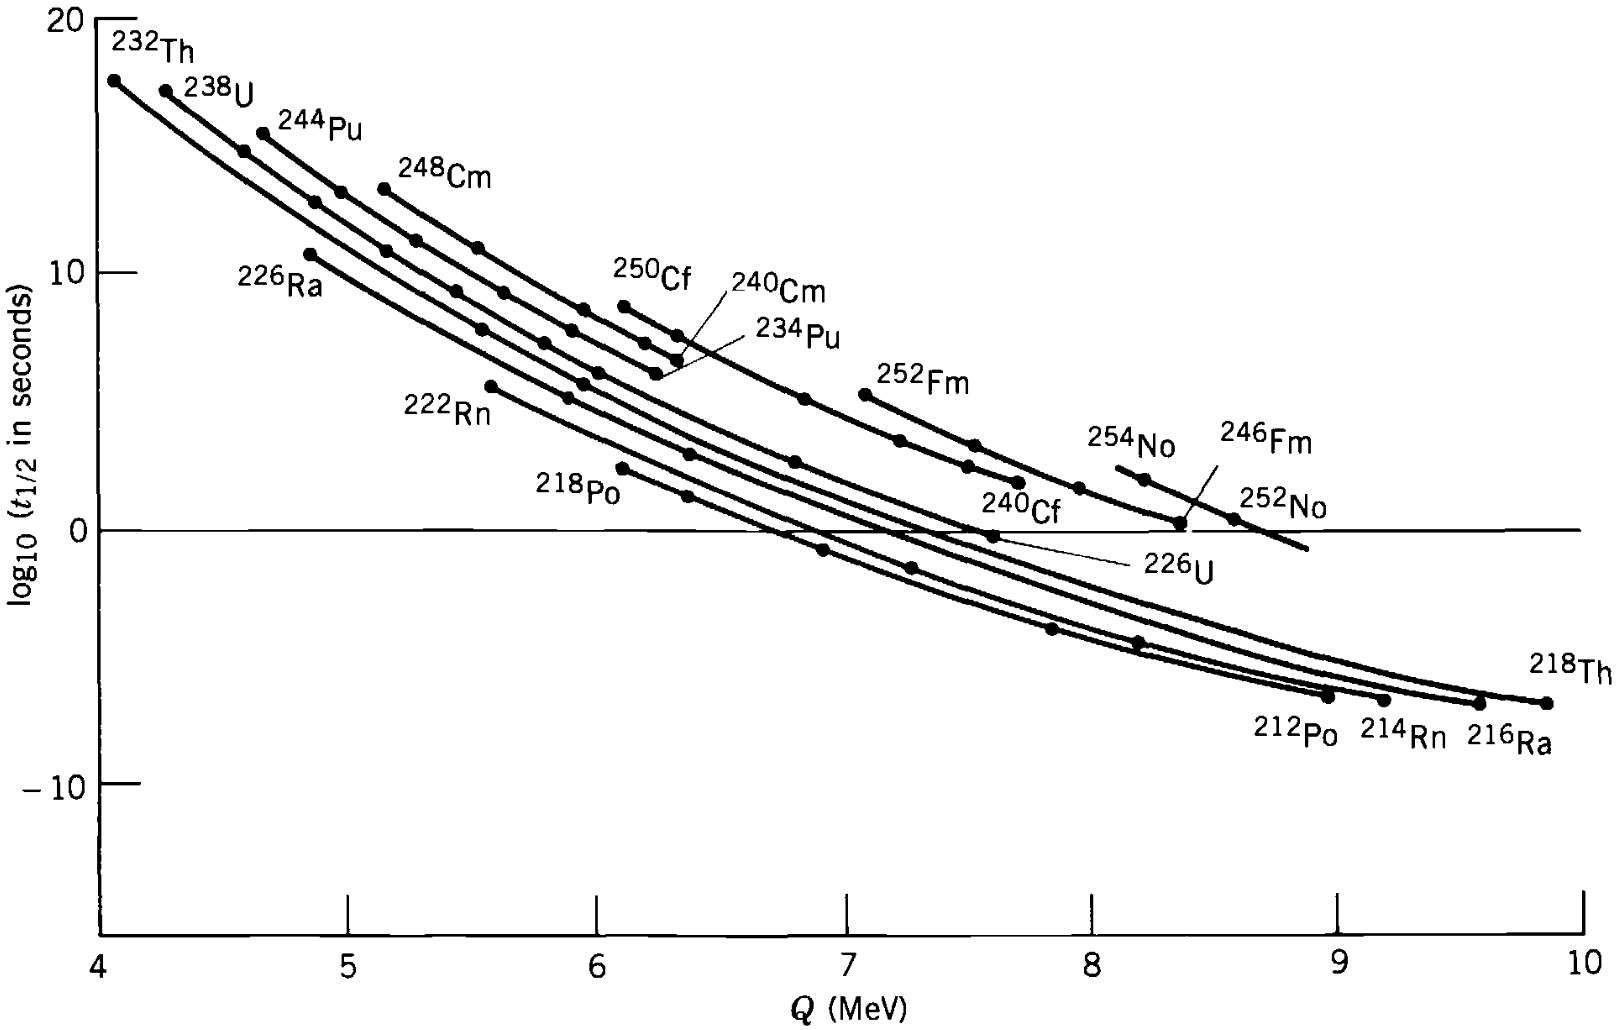
\includegraphics[width=0.75\textwidth]{geiger-nuttall.png}
	\caption{Legge di Geiger-Nuttal in famiglie isotopiche con nuclidi pari-pari.}
	\label{geiger-nuttall}
\end{figure}
\begin{figure}
	\centering
	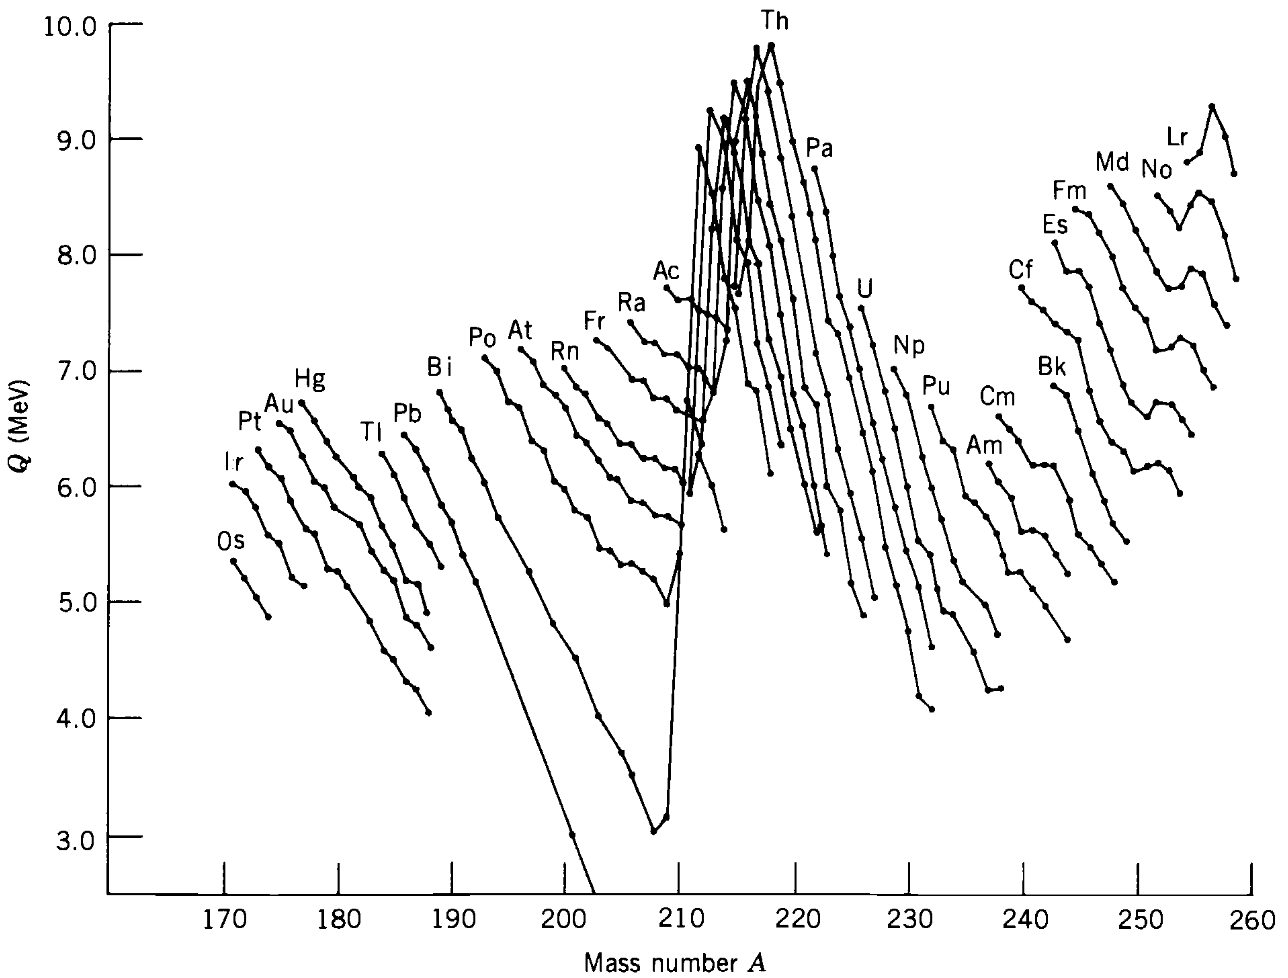
\includegraphics[width=0.75\textwidth]{gn-mass.png}
	\caption{Energia emessa per decadimento $ \alpha $ in famiglie isotopiche.}
	\label{gn-mass}
\end{figure}

\subsection{Teoria di Gamow}

La prima interpretazione teorica del decadimento $ \alpha $ fu data da Gamow nel 1929, qualche anno dopo le osservazioni di Geiger e Nuttall.\\
È possibile pensare alla particella $ \alpha $ come un corpo stabile preformato all'interno del nuclide $ \ch{^A X} $ che periodicamente di viene a trovare sulla superficie del nucleo, ad una distanza $ R \equiv R_{\ch{Y}} + R_{\alpha} $. Il moto della particella $ \alpha $ è determinato dal'energia potenziale d'interazione col nucleo, plottata in Fig. \ref{alpha-pot}, che fu proposta da Gamow essere:
\begin{equation}
	U(r) =
	\begin{cases}
		-V_0 & r < R \\
		\frac{2(Z-2)e^2}{4\pi \epsilon_0 r} & r > R
	\end{cases}
	\label{eq:2.12}
\end{equation}
Il senso fisico di tale espressione è che in prossimità del nucleo a prevalere è la forza nucleare, che ha natura attrattiva, mentre allontanandosi da esso prevale l'interazione coulombiana, che è repulsiva: si vede quindi la presenza di una barriera coulombiana in $ r = R $.\\
Con una trattazione classica la particella $ \alpha $ sarebbe emessa solo se $ E_{\alpha} > U(R) $ e ciò avverrebbe in un tempo comparabile al tempo di attraversamento del nucleo, ovvero $ t \sim R / v_{\alpha} = R \sqrt{2E_{\alpha} / m_{\alpha}} $: stimando $ R \approx 1.2\fm \left( (A - 4)^{1/3} + 4^{1/3} \right) $, per un nucleo con $ A \sim 230 $ e $ Q \sim 4\mev $ si trova $ R \sim 9\fm $ e $ t \sim 10^{-21}\,\text{s} $, ovvero un decadimento praticamente istantaneo. Ciò però non è quello che si osserva sperimentalmente.\\
Quantisticamente, invece, grazie all'effetto tunnel è possibile che anche le particelle $ \alpha $ con $ E_{\alpha} < U(R) $ (cosa che è praticamente sempre, dato che $ U(R) \sim 20\mev $) possono essere emesse con probabilità inderiori e dunque tempi di decadimento più lunghi.\\
È possibile svolgere il calcolo esplicitamente approssimando il potenziale coulombiano tra $ r = R $ ed $ r = R_{\alpha} $ (determinato da $ U(R_{\alpha}) = E_{\alpha} $) come una successione di barriere di potenziale di spessore $ dr $: dalla meccanica quantistica è noto che un'onda (particella) incidente su una barriera di potenziale di spessore $ L $ risulta in un'onda riflessa ed una trasmessa, le cui rispettive distribuzioni di probabilità (funzioni d'onda) sono determinate dai coefficienti di riflessione e trasmissione.

\begin{figure}[!hb]
	\centering
	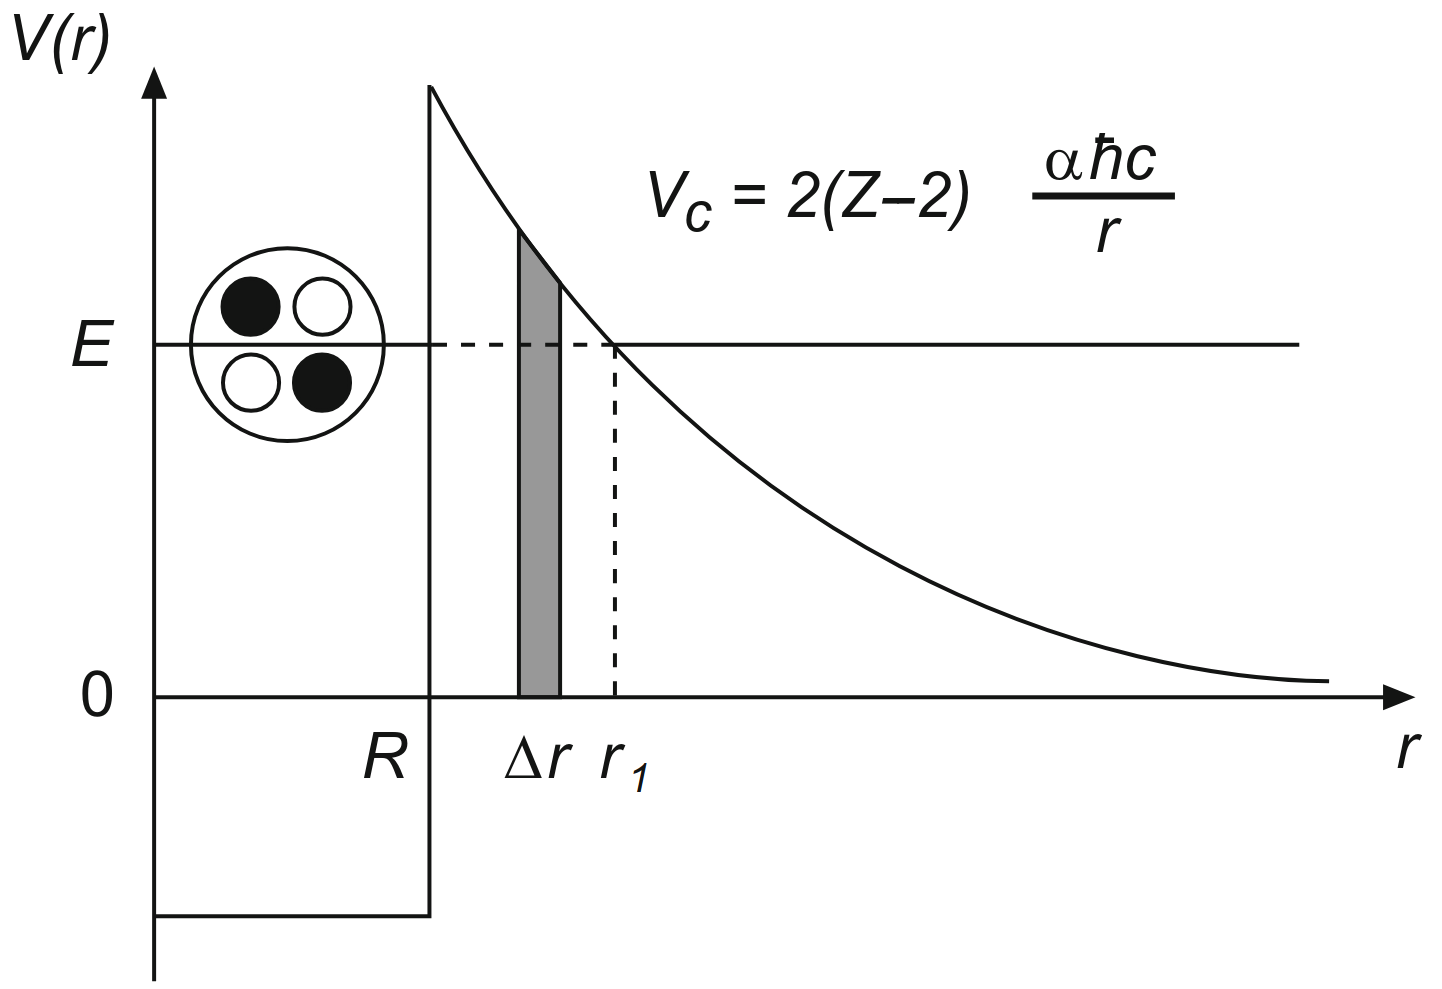
\includegraphics[width=0.60\textwidth]{alpha-pot.png}
	\caption{Potenziale d'interazione per il decadimento $ \alpha $.}
	\label{alpha-pot}
\end{figure}

Nel caso del decadimento $ \alpha $ è d'interesse solo il coefficiente di trasmissione nell'approssimazione $ E \ll V_0 $:
\begin{equation}
	T(E) = \left[ 1 + \frac{U_0^2}{4E (U_0 - E)} \sinh^2 \left( \frac{L}{\hbar} \sqrt { 2m (U_0 - E)} \right) \right]^{-1} \approx \frac{16 E (U_0 - E)}{U_0^2} e^{-2 \frac{L}{\hbar} \sqrt{2m (U_0 - E)}}
	\label{eq:2.13}
\end{equation}
Nel modello approssimato della successione di barriere di potenziale, quindi, si trova una probabilità di tunneling data da:
\begin{equation}
	P(E_{\alpha}) = \exp{\left[ -2 \int_{R}^{R_{\alpha}} dr \frac{1}{\hbar} \sqrt{2 m (U(r) - E_{\alpha}}) \right]} \eqdef e^{-2G}
	\label{eq:2.14}
\end{equation}
dove è stato definito il \textit{fattore di Gamow} $ G $. Svolgendo il calcolo col potenziale in Eq. \ref{eq:2.12} ed approssimando per una thick barrier $ R_{\alpha} \gg R $ (equivalente a $ E_{\alpha} \ll U(R) $, dato che dalla definizione $ R / R_{\alpha} = E_{\alpha} / U(R) $):
\begin{equation}
	\begin{split}
		G(E_{\alpha})
		&= \frac{2 (Z - 2) e^2}{\hbar} \sqrt{\frac{2m_{\alpha}}{E_\alpha}} \left[ \arccos \sqrt{\frac{R}{R_{\alpha}}} - \sqrt{\frac{R}{R_{\alpha}} - \frac{R^2}{R^2_{\alpha}}} \right]\\
		&\approx \frac{2 (Z - 2) e^2}{\hbar} \sqrt{\frac{2m_{\alpha}}{E_{\alpha}}} \left( \frac{\pi}{2} - \sqrt{\frac{R}{R_{\alpha}}} \right)
	\end{split}
	\label{eq:2.15}
\end{equation}
Questa espression mostra bene la fortissima dipendenza della probabilità di decadimento dall'energia della particella $ \alpha $: una piccola variazione di $ E_{\alpha} $ può portare $ P(E_{\alpha}) $ a variare di vari ordini di grandezza.\\
È anche possibile ricavare la legge di Geiger-Nuttall, dato che fenomenologicamente di può scrivere:
\begin{equation}
	\lambda = S \nu P(E_{\alpha})
	\label{eq:2.16}
\end{equation}
dove $ \lambda $ è la costante di decadimento, $ S $ è la probabilità che si formi una particella $ \alpha $ nel nucleo (può essere presa $ S \approx 1 $) e $ \nu $ è la knocking frequency, ovvero la frequenza con cui la particella $ \alpha $ urta con la barriera coulombiana. Si può stimare $ \nu $ a partire dal tempo che impiega la particella $ \alpha $ ad attraversare il nucleo (già trovato in precedenza): $ \nu \sim t^{-1} \sim 10^{21} \,\text{Hz} $. Dall'Eq. \ref{eq:2.16} si ha:
\begin{equation}
	\ln \lambda = \ln S + \ln \nu - 2 G(E_{\alpha}) \sim a(Z) - b \frac{Z}{\sqrt{E_{\alpha}}}
	\label{eq:2.17}
\end{equation}
che, ricordando che $ t_{1/2} = \frac{\ln 2}{\lambda} $, è proprio la legge di Geiger-Nuttall.\\
Ovviamente tutte queste relazioni sono qualitative e non quantitative, dato che sono state fatte alcune approssimazioni dalle quali la realtà si discosta notevolmente, prima su tutti la simmetria sferica: i nuclidi pesanti hanno forme notevolmente deformate (tendenti ad ellissoidi di rotazione), dunque le loro emissioni presentano notevoli anisotropie nella distribuzione angolare di particelle $ \alpha $.

\subsection{Spettri}

Per molti nuclidi che decadono tramite decadimento $ \alpha $ è possibile la presenza di più branch di decadimento, con percentuali di decadimento basse rispetto a quella dominante, che non portano direttamente allo stato fondamentale del nucleo figlio, ma a qualche suo stato eccitato: ciascuna di queste branch ha una propria energia di decadimento (deve essere sempre mono-energetico), e solitamente la branch con l'energia più alta è quella che va a popolare lo stato fondamentale del nucleo figlio.\\
Lo studio degli spettri di decadimento così prodotti (ad esempio immettendo le particelle $ \alpha $ in uno spettrometro magnetico) è importante per studiare i vari livelli energetici del nucleo figlio, specialmente nel caso in cui esso appartenga ad una specie nucleare di difficile sintesi.

\subsection{Cluster decay}

Spesso, quando un nuclide risulta instabile rispetto al decadimento per $ \ch{^4 He} $, esso lo è anche rispetto a quello per $ \ch{^8_4 Be} $, $ \ch{^{12}_6 C} $ ed altri nuclei, tendenzialmente formati da più particelle $ \alpha $, i cosiddetti \textit{nuclear clusters}. Anche questi sono sistemi particolarmente stabili preformati nel nucleo e, per un nuclear cluster di $ n $ particelle $ \alpha $, si può approssimare $ Q_n \sim Q_{\alpha}^n $: di conseguenza, per la legge di Geiger-Nuttall, i tempi di decadimento sono enormemente più lungi rispetto a quelli del decadimento $ \alpha $, con conseguenza che i branching ratios sono praticamente trascurabili, sebbene occasionalmente questi cluster decays vengano osservati e siano stati ampiamente studiati.

\section{Fissione}

Dopo la scoperta del neutrone da parte di Chadwick nel 1932, furono condotti numerosi esperimenti nei quali vari nuclidi venivano irraggiati con neutroni: in particolare, Fermi et al. studiarono la radioattività a seguito della neutron capture, ottenendo il Nobel nel 1938 per gli studi sul decadimento $ \beta^- $, mentre Meitner e Hahn osservarono la fissione negli elementi transuranici.

\paragraph{Neutroni}

Si utilizza una specifica terminologia per classificare i neutroni in base alla loro energia $ E_n $:
\begin{enumerate}
	\item high energy neutrons: $ E_n > 100\mev $;
	\item fast neutrons: $ 100\kev < E_n < 100\mev $;
	\item epithermal neutrons: $ 0.1\ev < E_n < 100\kev $;
	\item thermal/slow neutrons: $ 1\,\text{meV} < E_n < 0.1\ev $,
	\item cold/ultracold neutrons: $ E_n < 1\,\text{meV} $.
\end{enumerate}
Come si può vedere in Fig. \ref{fission-cs}, sperimentalmente si trova che i neutroni a basse energie, specialmente i thermal neutrons, sono quelli più efficaci per indurre reazioni di fissione nucleare.

\begin{figure}
	\centering
	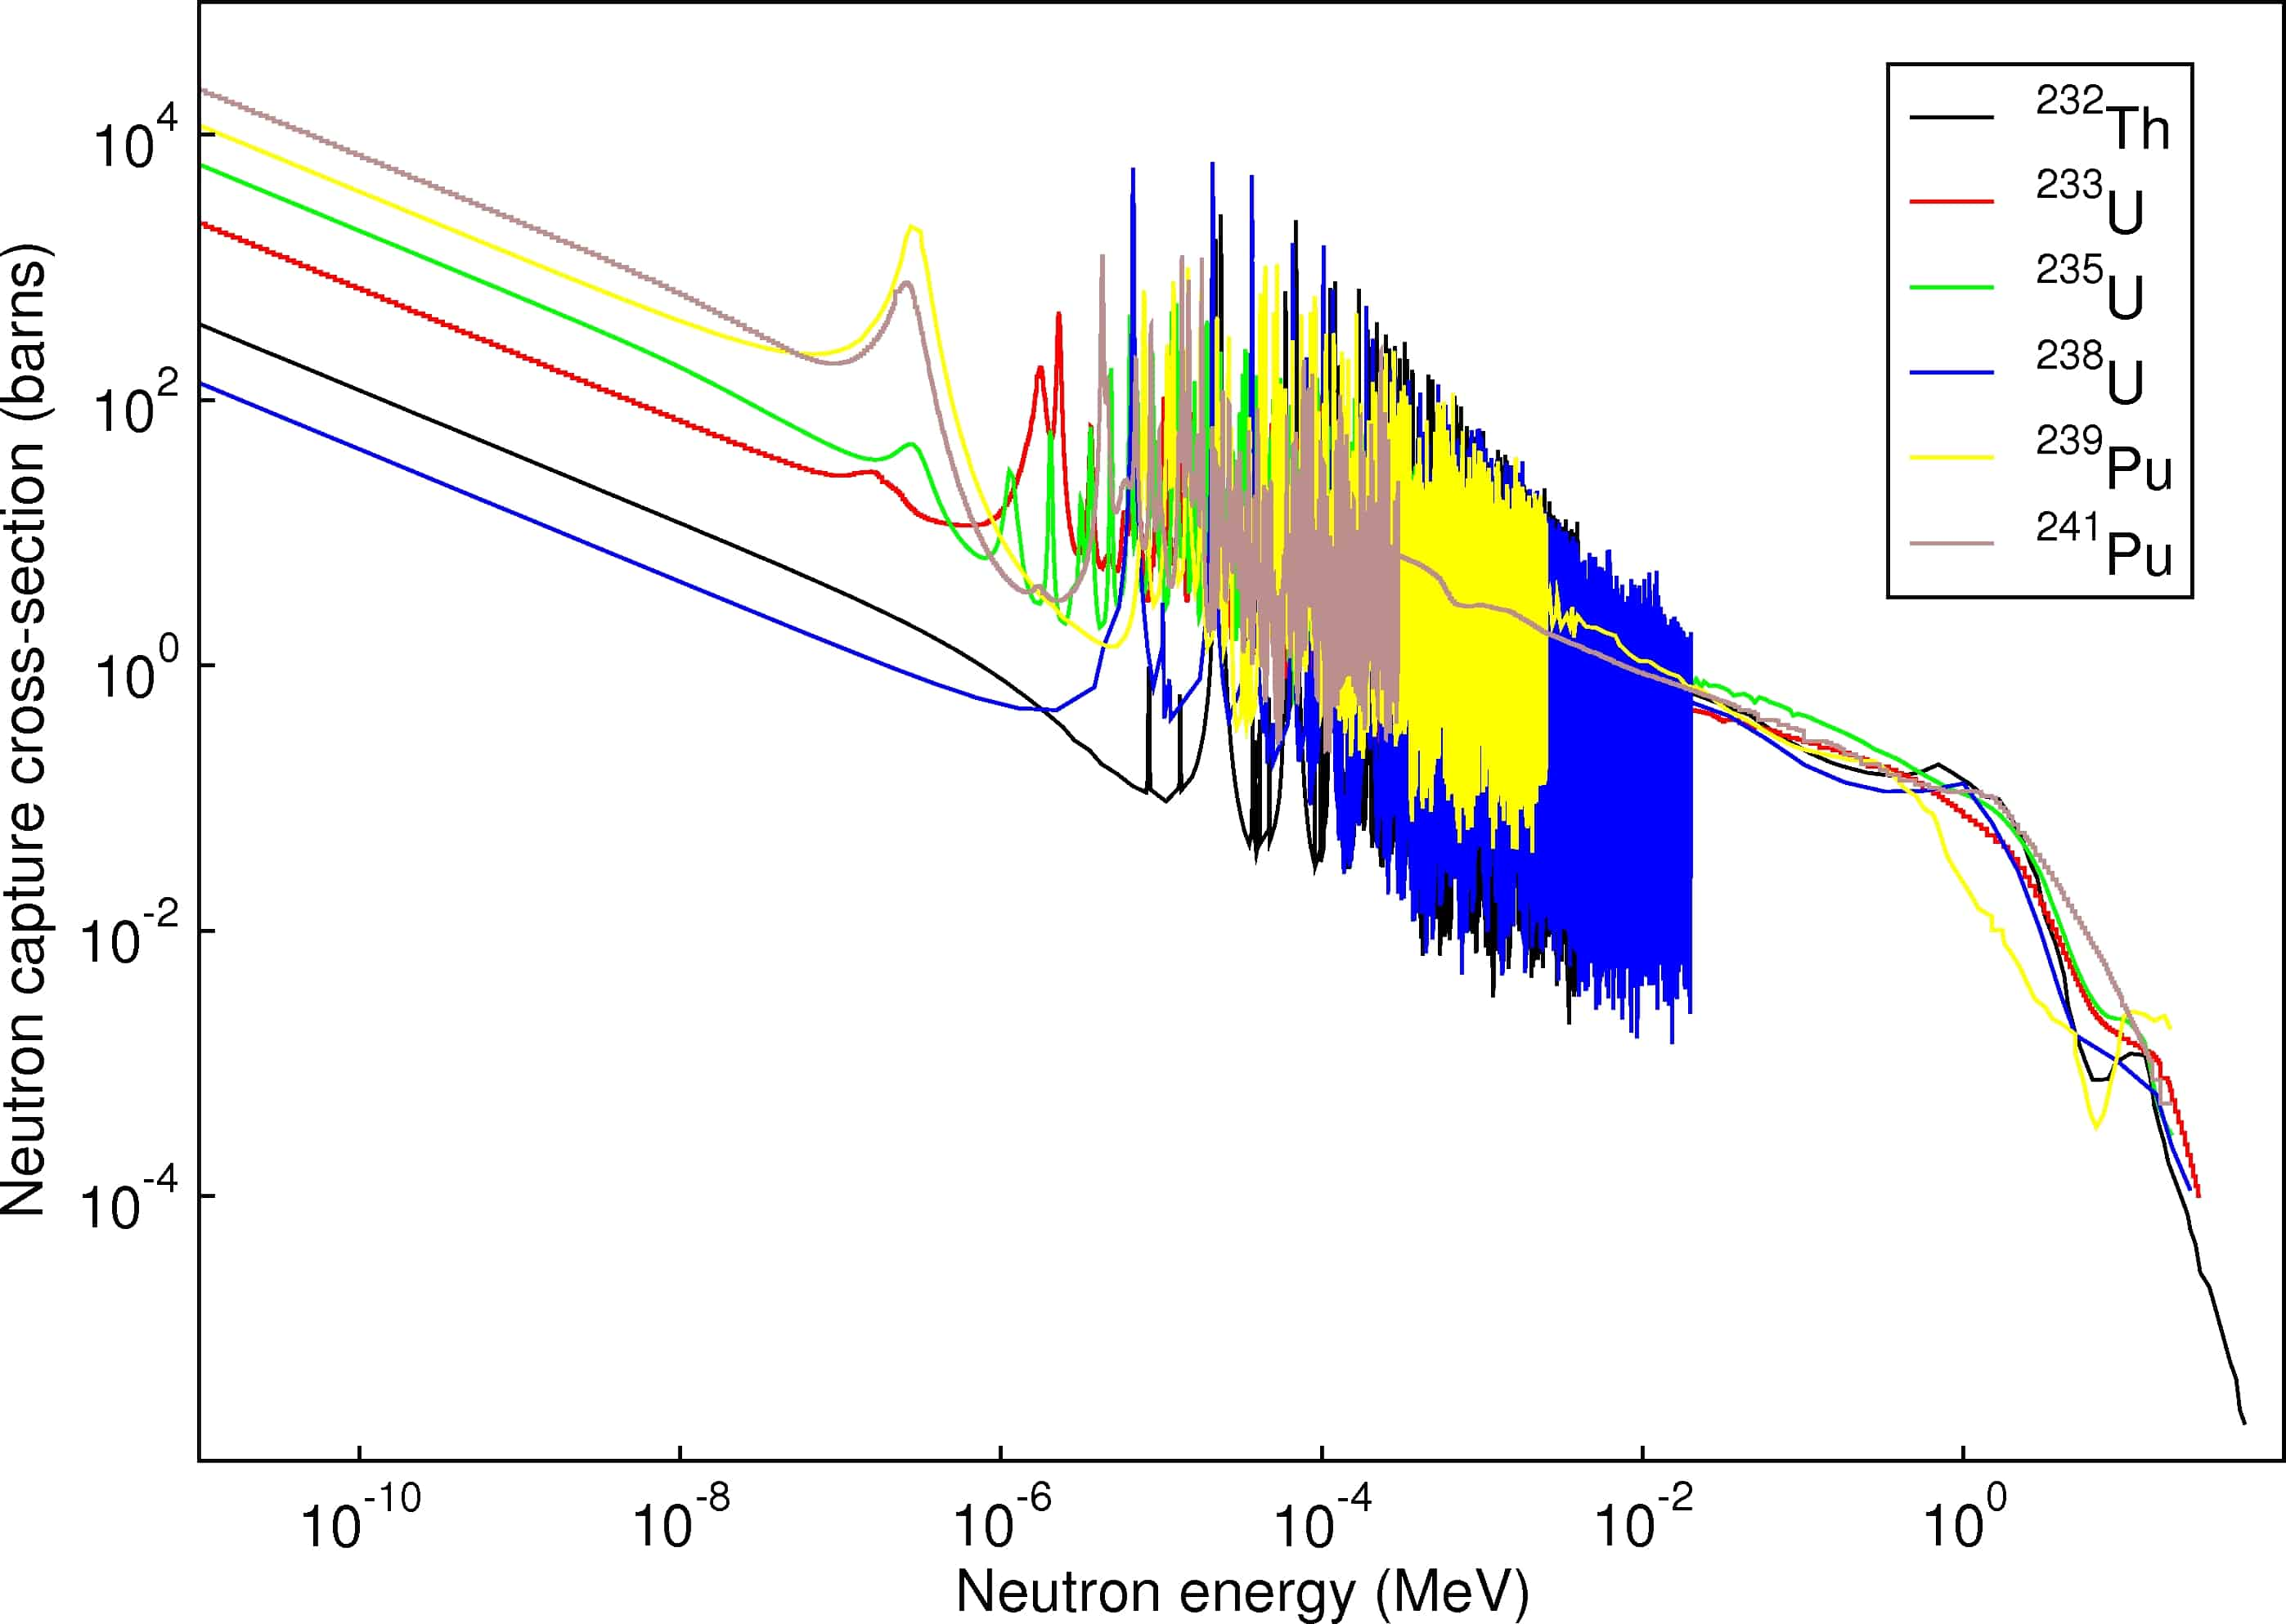
\includegraphics[width=0.75\textwidth]{fission-cs.jpg}
	\caption{Neutron-induced fission cross-section.}
	\label{fission-cs}
\end{figure}
\begin{figure}
	\centering
	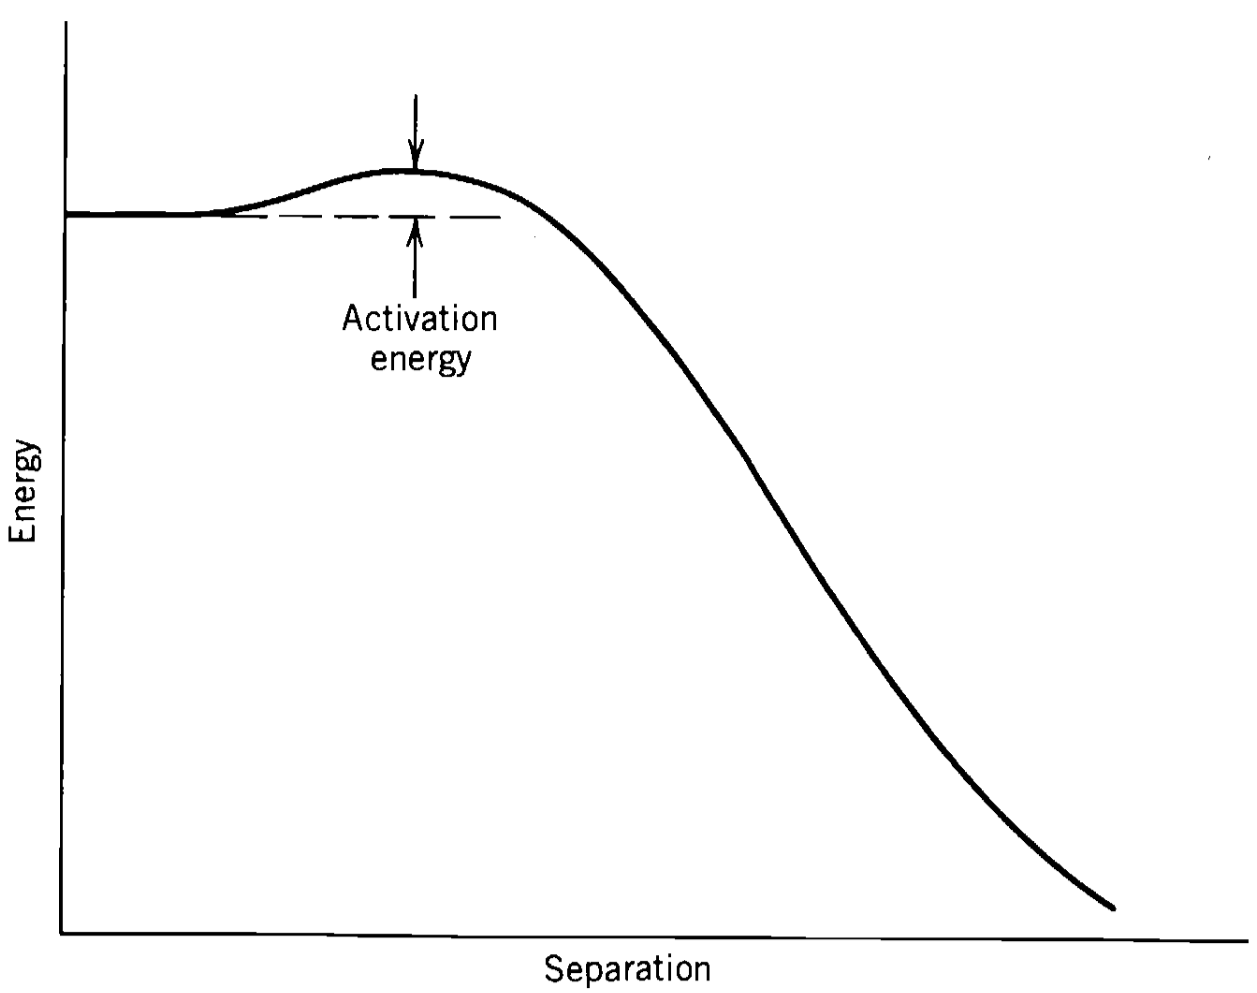
\includegraphics[width=0.75\textwidth]{fission-pot.png}
	\caption{Coulomb potential in a fissioning nucleus.}
	\label{fission-pot}
\end{figure}

\subsection{Fissione spontanea}

La tendenza dei nuclei pesanti a fissionare è evidente dall'andamento della binding energy rispetto ad $ A $ (Fig. \ref{bind-en}): ad esempio, se si considera la fissione dell'uranio $ \ch{^{235}_{92} U} \rightarrow \ch{^{90}_{36} Kr} + \ch{^{142}_{56} Ba} + 3 n $, il $ Q $-value della reazione è $ 166.73\mev $, dunque è una reazione energeticamente fortemente favorita. Va però notato che il decay branch per decadimento $ \alpha $ è fortemente dominante in natura, basta confrontare, ad esempio, i seguenti decadimenti:
\begin{equation*}
	\begin{split}
		\ch{^{238}_{92} U} \xrightarrow{4\,\text{Gy}} \ch{^{234}_{90} Th} + \alpha &\qquad \ch{^{238}_{92} U} \xrightarrow{\sim 10^7\,\text{Gy}} \ch{^{140}_{54} Xe} + \ch{^{96}_{38} Sr} + 2n\\
		\ch{^{235}_{92} U} \xrightarrow{0.7\,\text{Gy}} \ch{^{231}_{90} Th} + \alpha &\qquad \ch{^{235}_{92} U} \xrightarrow{\sim 10^8\,\text{Gy}} \ch{^{142}_{56} Ba} + \ch{^{90}_{36} Kr} + 3n
	\end{split}
\end{equation*}
La fissione è osservata solo in nuclei pesanti (il nuclide fissile più leggero è $ \ch{^{226}_{88} Ra} $), e la fissione spontanea diventa il decay mode dominante solo in nuclidi con $ A \ge 250 $.\\
Ciò che inibisce la fissione è una barriera coulombiana analoga a quella del decadimento $ \alpha $: in questo caso, però, essa ha un andamento liscio (in senso analitico), com'è possibile vedere in Fig. \ref{fission-pot}. L'energia necessaria affinché i due prodotti della fissione (supposti preformati) oltrepassino la barriera coulombiana è, nella maggior parte dei casi, troppo alta per rendere la fissione un decay mode significativo; a livello teorico, dovrebbero esistere anche dei nuclidi in cui la barriera si annulla, ovvero in cui i due prodotti hanno sempre l'energia necessaria per superarla, e tali nuclidi dovrebbero fissionare istantaneamente: naturalmente essi non esistono in natura, e si dovrebbero trovare attorno ad $ A = 300 $.\\
L'altezza della barriera coulombiana rispetto all'energia del ground state è detta activation energy ed è possibile calcolarla sia assumendo il modello semplificato a goccia sia tenendo conto degli effetti delle shell nucleari: entrambi i casi sono pllottati in Fig. \ref{act-en}.

\begin{figure}
	\centering
	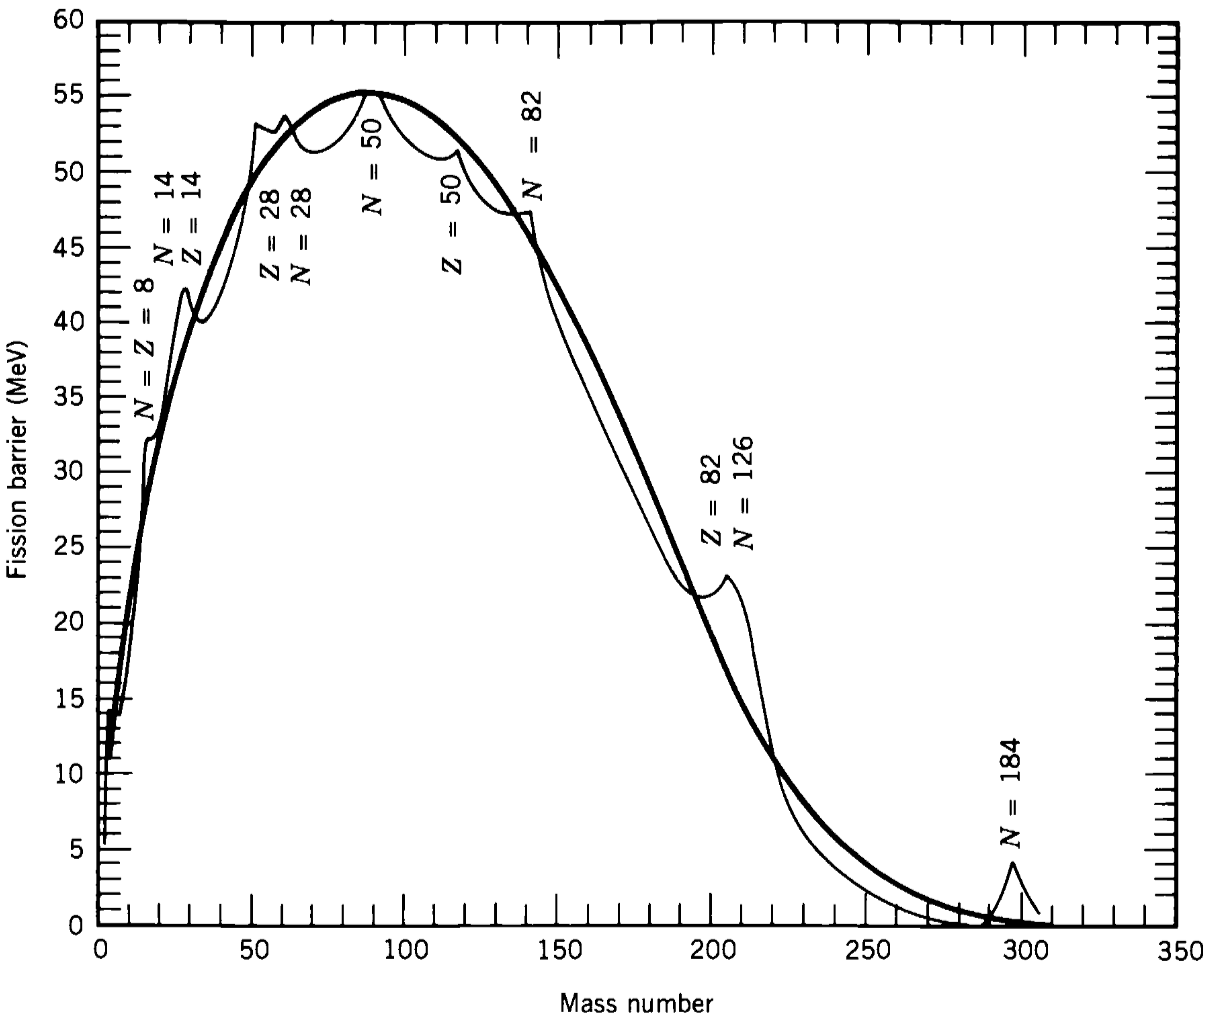
\includegraphics[width=0.65\textwidth]{act-en.png}
	\caption{Activation energy of nuclear fission.}
	\label{act-en}
\end{figure}
\begin{figure}
	\centering
	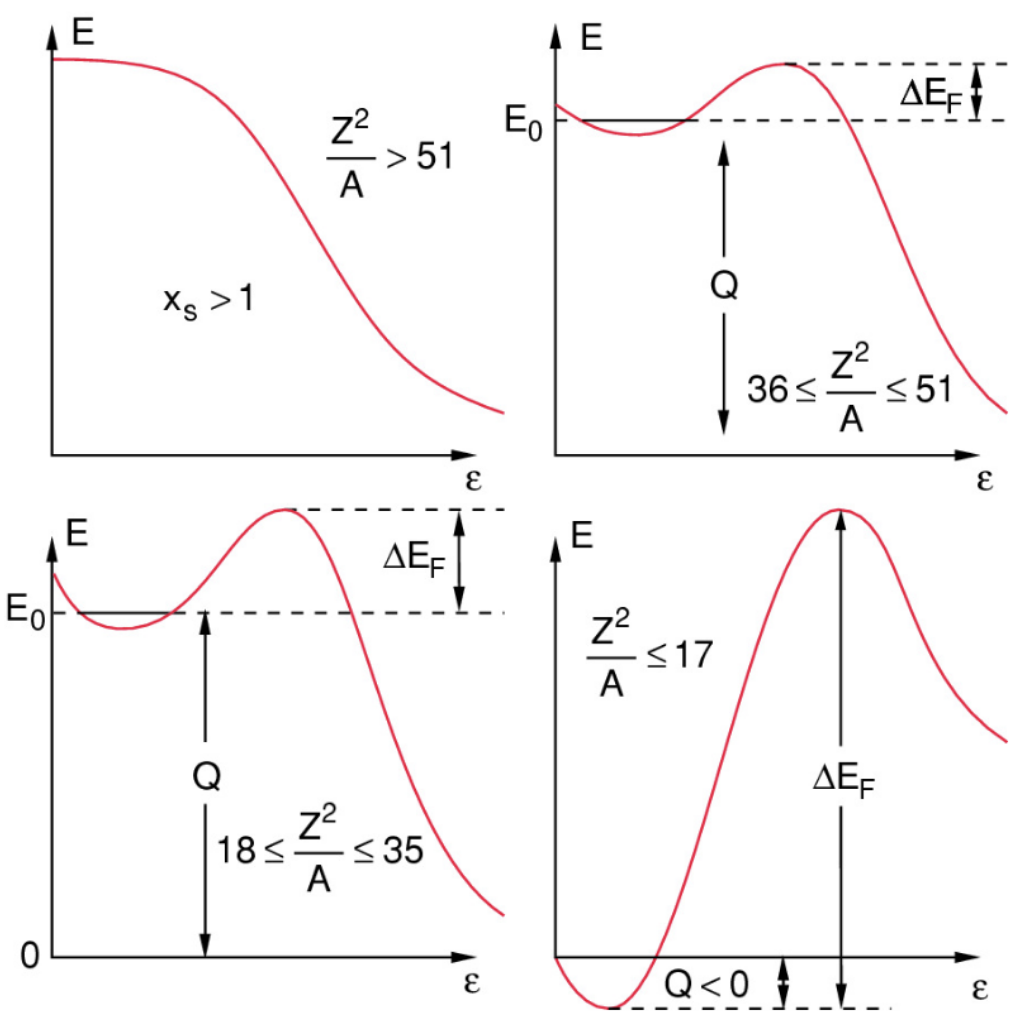
\includegraphics[width=0.60\textwidth]{act-en-z.png}
	\caption{Potential barrier as a funzion of the deformation parameter for various fissility values.}
	\label{act-en-z}
\end{figure}

\paragraph{Liquid drop model}

Semplificando, questo modello considera solo le proprietà nucleari medie, assumendo un nuclide sferico nel suo ground state. Nel caso di un nucleo fissile, l'instabilità porta ad una deformazione del nuclide in un ellissoide: assumendo il raggio iniziale $ R $ e l'eccentricità dell'ellissoide $ \varepsilon $, si possono calcolare i semiassi come:
\begin{equation}
	a = R \left( 1 + \varepsilon \right) \qquad b = R \left( 1 + \varepsilon \right)^{-1/2}
	\label{eq:2.18}
\end{equation}
Si vede dunque che il volume $ V = \frac{4}{3}\pi R^3 = \frac{4}{3} \pi ab^2 $ rimane inalterato, mentre la superficie varia di un fattore approssimabile ad $ \varepsilon $: $ S = 4\pi R^2 \left( 1 + \frac{2}{5} \varepsilon^2 + \dots \right) $; analogamente, si mostra che l'energia d'interazione coulombiana varia di un fattore $ \left( 1 - \frac{1}{5} \varepsilon^2 + \dots \right) $.\\
Dalla formula semi-empirica di Weizsäcker (Eq. \ref{eq:1.30}) deriva che, a seguito della deformazione, la binding energy varia di:
\begin{equation}
	\Delta B = - a_S A^{2/3} \left( 1 + \frac{2}{5} \varepsilon^2 + \dots \right) - a_C \frac{Z^2}{A^{1/3}} \left( 1 - \frac{1}{5} \varepsilon^2 + \dots \right) \approx \left( -\frac{2}{5} a_S A^{2/3} + \frac{1}{5} a_C \frac{Z^2}{A^{1/3}} \right) \varepsilon^2
	\label{eq:2.19}
\end{equation}
Se $ \Delta B > 0 $, il nucleo risulta instabile rispetto alla deformazione e fissiona, dunque si trova una condizione per la fissione spontanea:
\begin{equation}
	\Chi \defeq \frac{a_C}{2a_S} \frac{Z^2}{A} > 1
	\label{eq:2.20}
\end{equation}
dove è stata definita la fissility $ \Chi $. Utilizzando i valori di $ a_S $ ed $ a_C $ interpolati si trova la condizione $ Z^2 / A > 51 $, ovvero $ Z > 114 $ e $ A > 270 $; al di sotto di questi valori la fissione è possibile solo fornendo la necessaria energia di attivazione (vedere Fig. \ref{act-en-z}).\\
Bisogna specificare che per $ Z^2 / A > 51 $ la fissione spontanea è istantanea, mentre per nuclidi con $ Z^2 / A \lesssim 51 $ è possibile anche una delayed fission per effetto tunnel (a causa della repulsione tra protoni), analogamente al decadimento $ \alpha $, ma nella maggior parte dei casi quest'ultimo è dominante.
Infine, si può notare in Fig. \ref{fission-lt} come i tempi di decadimento aumentino al diminuire di $ Z^2 / A $.

\begin{figure}[!hb]
	\centering
	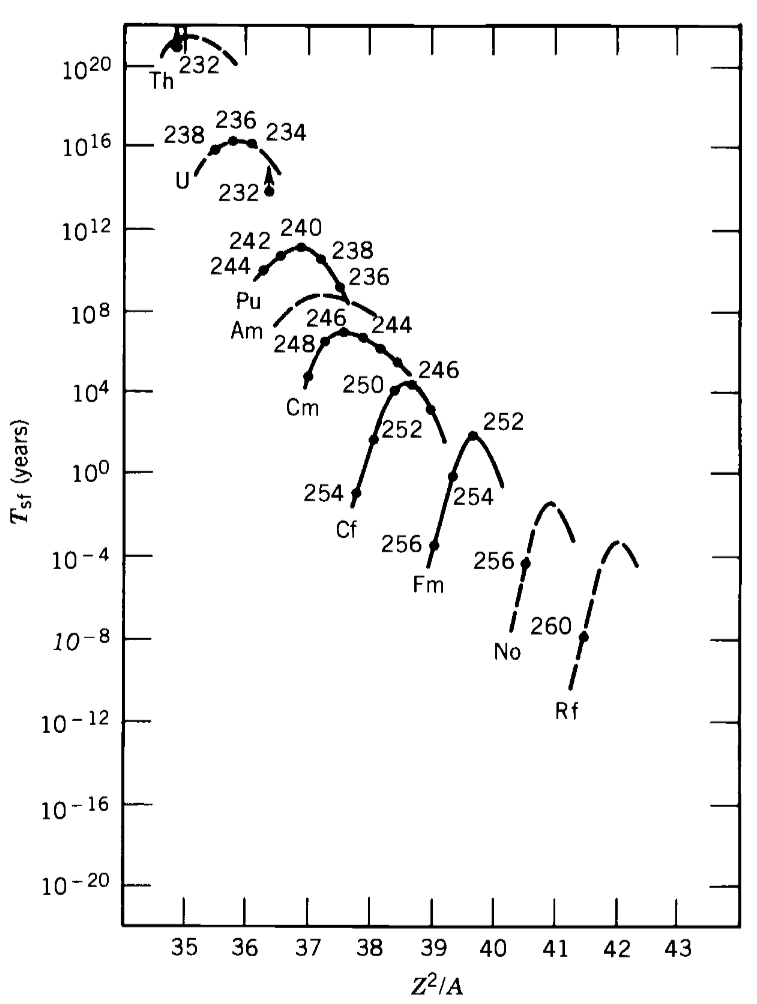
\includegraphics[width=0.80\textwidth]{fission-lt.png}
	\caption{Lifetimes for spontaneous fission.}
	\label{fission-lt}
\end{figure}

\subsection{Fissione indotta}

Dato che i neutroni non sono affetti dal potenziale coulombiano, è possibile indurre la fissione di un nuclide facendolo scatterare con un neutrone termico. Bisogna però notare una differenza tra la fissione di nuclidi pari-pari e nuclidi pari-dispari, dovuta al termine di pairing nella formula di Weizsäcker (Eq. \ref{eq:1.30}).\\
Si considerino ad esempio due campioni di $ \ch{^{235}_{92} U} $ e $ \ch{^{235}_{92} U} $ e li si irraggi con neutroni termici:
\begin{enumerate}
	\item $ \ch{^{235}_{92} U} + n \rightarrow \ch{^{236}_{92} U}^* $: $ Q = 6.5\mev > \Delta E_F = 6.1\mev $;
	\item $ \ch{^{238}_{92} U} + n \rightarrow \ch{^{239}_{92} U}^* $: $ Q = 4.8\mev < \Delta E_F = 6.4\mev $;
\end{enumerate}
Si vede dunque che la fissione di $ \ch{^{235}_{92} U} $ può avvenire con neutroni termici, mentre per quella di $ \ch{^{238}_{92} U} $ sono necessari neutroni veloci. Ciò è dovuto al fatto che i nuclidi pari-pari sono energeticamente favoriti, dunque il termine di pairing favorisce processi da pari-dispari a pari-pari, mentre ostacola quelli da pari-pari a pari-dispari: nel caso considerato, infatti, la differenza di energia ammonta a $ \Delta E = \delta (236^{-1/2} + 238^{-1/2}) = 1.5\mev $.\\
È interessante notare che $ \ch{^{235}_{92} U} $ e $ \ch{^{238}_{92} U} $ sono gli unici isotopi dell'uranio rimasti in natura, con abbondanze isotopiche rispettivamente del $ 0.72\% $ e $ 99.28\% $.

\subsection{Caratteristiche}

Il processo di fissione del nuclide non presenza grosse differenze tra il caso spontaneo e quello indotto: in maniera quasi istantanea ($ \sim 10^{-17}\,\text{s} $) il nucleo si deforma radicalmente andando a formare i due frammenti di fissione (sono possibili fissioni ternarie ma sono estremamente rare), i quali si separano in tempi brevissimi ($ \sim 10^{-14}\,\text{s} $): questi sono nuclidi molto neutron-rich, dunque espellono i neutroni con energie di legame superiori all'energia di legame media, andando così a formare i prodotti di fissione; quest'ultimi possono decadere tramite decadimenti $ \beta $ e $ \gamma $, con tempi su una scala dai secondi ai milioni di anni, muovendosi verso la valle di stabilità.

\subsubsection{Asimmetria di fissione}

I due frammenti altamente eccitati in cui si separa il nucleo a seguito della fissione non sono uguali, ma presentano una notevole asimmetria; per di più, variando il nuclide fissile si osserva che la distribuzione dei frammenti pesanti rimane praticamente inalterata, mentre la massa in eccesso viene inglobata dai frammenti leggeri (vedere Fig. \ref{fission-md}).\\
Ciò può essere spiegato dal fatto che la fissione, sebbene trattata in maniera elementare utilizzando il liquid drop model, risente in realtà degli effetti delle shell nucleari: come si può notare in Fig. \ref{fission-asimm}, la distribuzione dei frammenti pesanti si sovrappone ad una regione di completamento di shell nucleari, con la presenza anche del nuclide doubly-magic $ \ch{^{132}_{50} Sn_{82}} $, che ha una configurazione estremamente stabile; tutto ciò non accade, invece, per la distribuzione dei frammenti leggeri, i quali non si sovrappongono a nessun magic nucleus.\\
Circa metà dei prodotti di fissione decadono in meno di un anno, mentre i restanti possono avere tempi di decadimento anche di milioni di anni: questi formano le scorie radioattive.\\
I prodotti di fissione sono molto neutron-rich, dunque per la maggior parte sono instabili per decadimento $ \beta^- $: la fissione nucleare è un importante strumento di ricerca per la regione $ \beta^- $-instabile, difficilmente raggiungibile con altri metodi: i prodotti di fissione possono dar luogo ad intere catene di decadimenti $ \beta^- $.

\begin{figure}
	\centering
	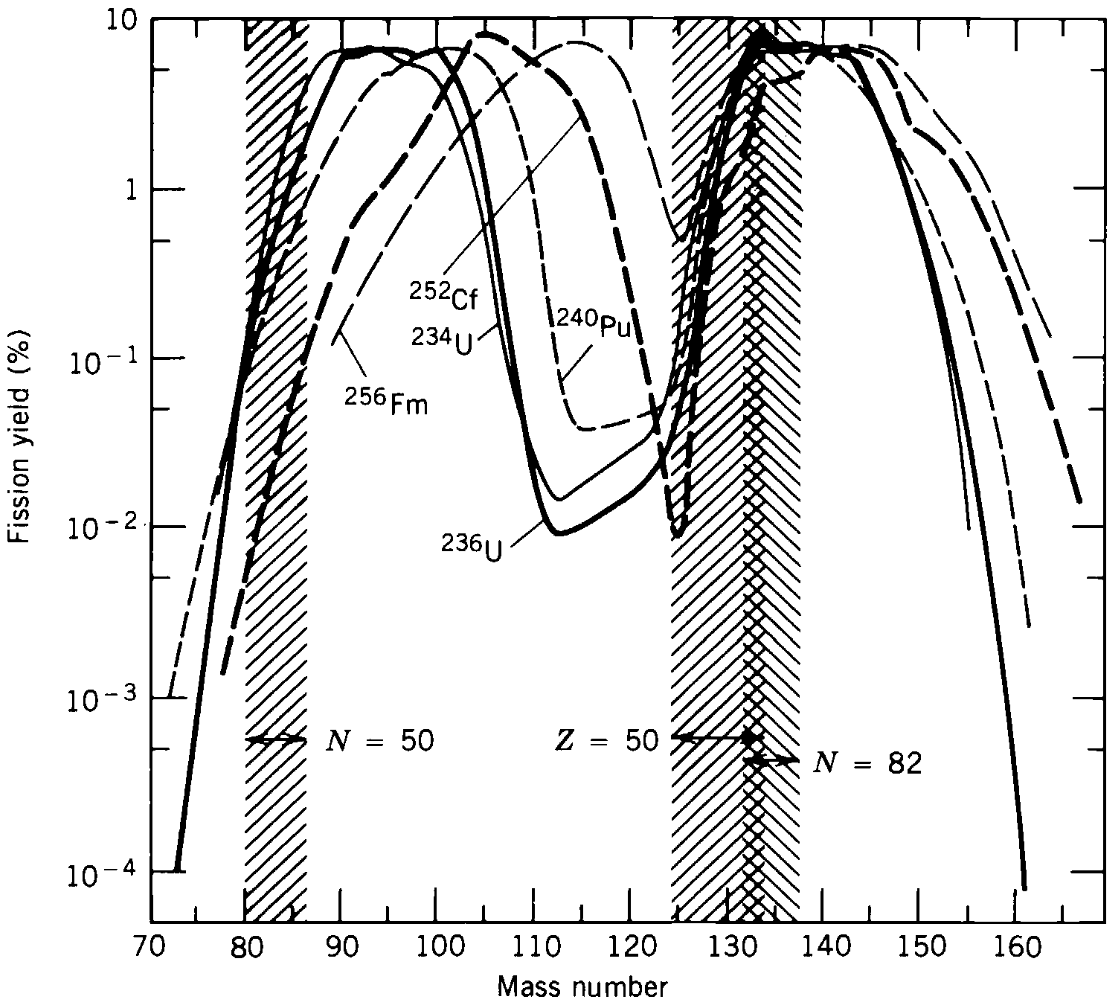
\includegraphics[width=0.60\textwidth]{fission-asimm.png}
	\caption{Asimmetry in fission products.}
	\label{fission-asimm}
\end{figure}
\begin{figure}
	\centering
	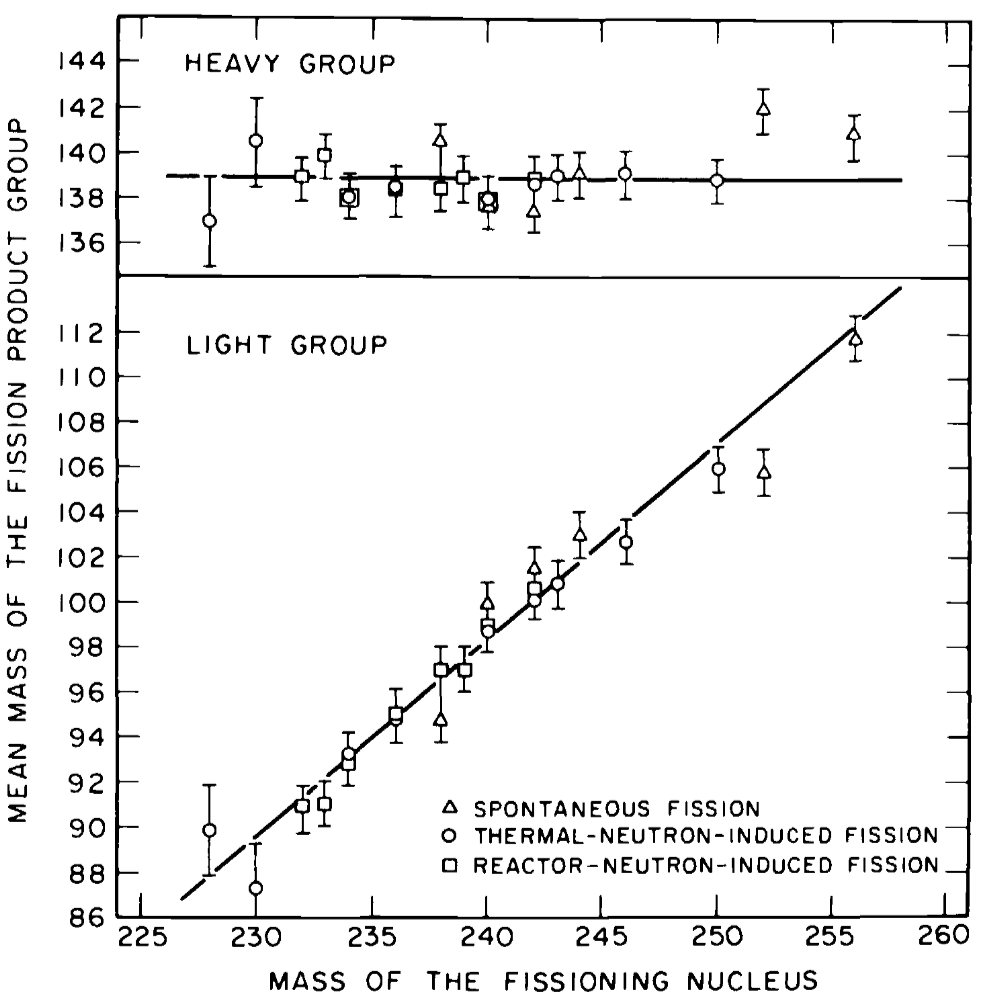
\includegraphics[width=0.60\textwidth]{fission-md.png}
	\caption{Distributions of light and heavy fission products.}
	\label{fission-md}
\end{figure}

\subsubsection{Emissione di neutroni}

I neutroni prodotti dalla fissione di un nuclide si possono distinguere in due categorie: prompt neutrons and delayed neutrons.\\
I prompt neutrons vengono emessi praticamente in contemporanea al processo di fissione, venendo emessi dal nuclide fissile e dai frammenti di fissione: il numero di prompt neutrons viene indicato come $ \nu_n $ e generalmente si ha $ \langle \nu_n \rangle \approx 2.4 $.\\
La distribuzione di prompt neutrons in base alla loro energia cinetica è una distribuzione di Maxwell, mentre $ \nu_n $ si distribuisce secondo una gaussiana indipendentemente dalla fissione considerata, come visibile in Fig. \ref{n-neut-dist}: i prompt neutrons vengono prodotti con energia di circa $ 2\mev $, in media.\\
I delayed neutrons, d'altro canto, sono quelli prodotti nelle decay chains iniziate dai prodotti di fissione, solitamente tra $ 0.2\,\text{s} $ e $ 60\,\text{s} $ dopo la fissione, e costituiscono appena l'$ 1\% $ dei neutroni totali prodotti dalla fissione.

\begin{figure}[!b]
	\centering
	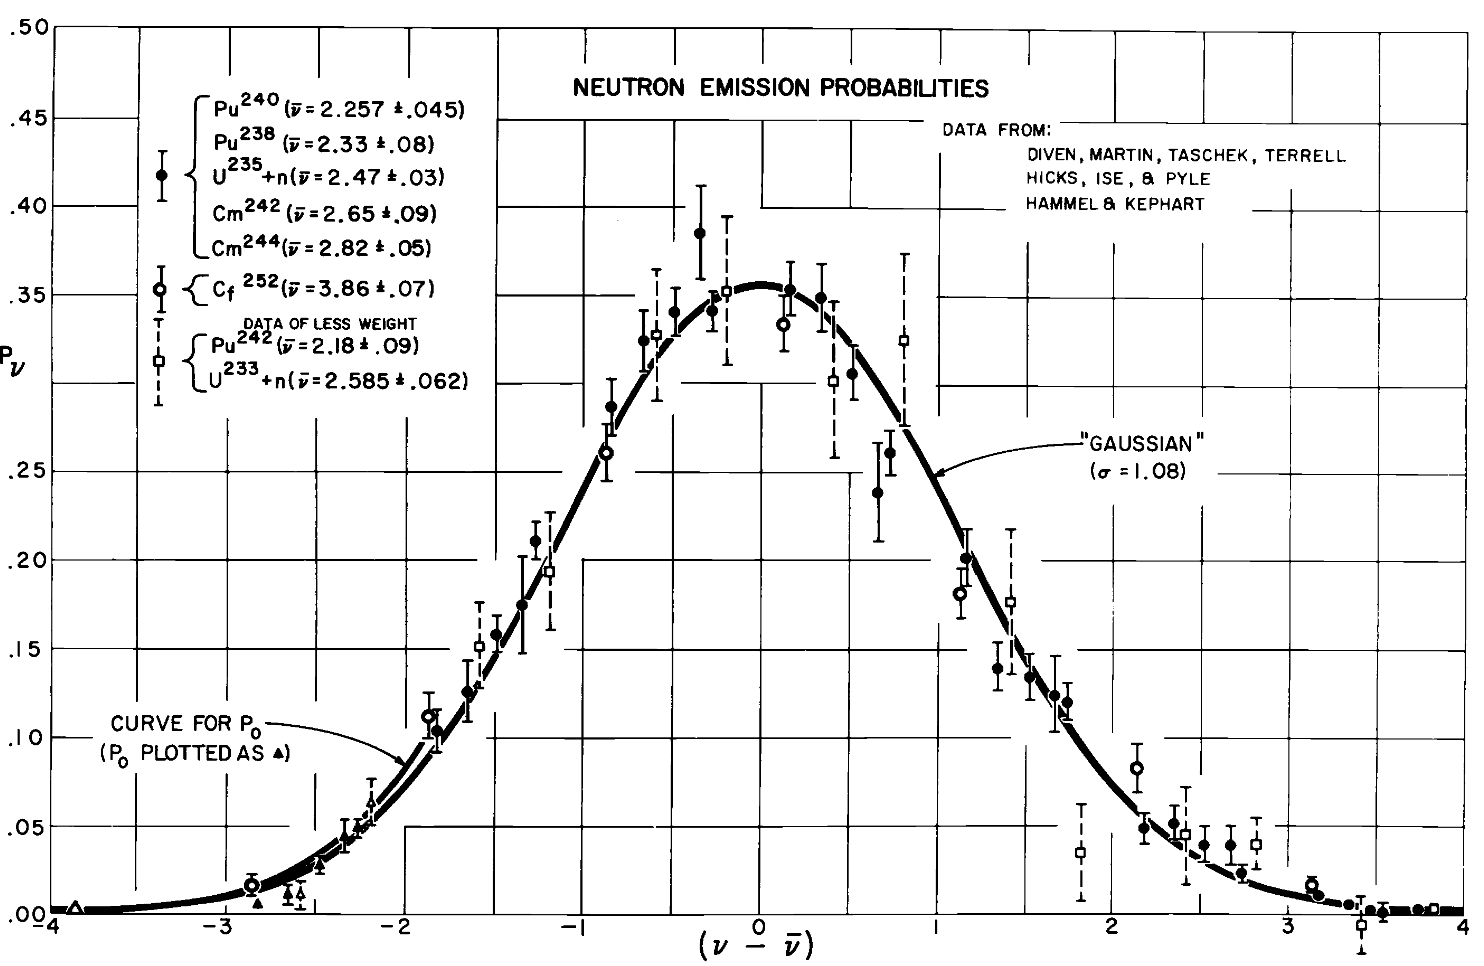
\includegraphics[width=0.75\textwidth]{n-neut-d.png}
	\caption{Prompt neutrons' number distribution.}
	\label{n-neut-dist}
\end{figure}

\subsubsection{Bilancio energetico}

Considerando, ad esempio, la fissione del $ \ch{^{235}_{92} U} $, i $ 210\mev $ di energia rilasciata vengono ripartiti nel seguente modo:
\begin{enumerate}
	\item frammenti di reazione: $ \ch{Y}_{\text{small}} \approx 100\mev $ e $ \ch{Y}_{\text{large}} \approx 70\mev $;
	\item prompt emissions: neutrons $ \approx 5\mev $ e fotoni $ \approx 7\mev $;
	\item decadimenti: $ \beta^- \approx 20\mev $ (di cui $ \approx 12\mev $ persi in neutrini) e $ \gamma \approx 8\mev $.
\end{enumerate}
La differenza tra i due frammenti è dovuta alla conservazione del momento lineare: trascurando i neutroni si ha $ m_1 \ve{v}_1 = m_2 \ve{v}_2 $, dunque $ K_1 / K_2 = m_2 / m_1 $, ovvero il frammento leggero acquista la maggior parte del'energia cinetica disponibile.

\subsection{Applicazioni}

\subsubsection{Studio della stuttura nucleare}

Dato che la fissione produce nuclidi neutron-rich eccitati molto esotici, essa può essere usata per studiare una zona difficilmente popolabile della nuclear chart, quella $ \beta^- $-instabile.\\
Inoltre, a partire dalla fissione è possibile ottenere la cosiddetta spallazione del nuclide fissile: quando il l'energia della particella proiettile è molto elevata la fissione produce frammenti multipli. Essendo il processo non più binario, la distribuzione dei frammenti non è più a doppia campana (come in Fig. \ref{fission-asimm}), ma si va a popolare anche la conca centrale: più è alta l'energia del proiettile, più saranno i frammenti di masse intermedie prodotti.\\
Questo, ad esempio, è ciò che avviene nell'esperimento ISOLDE al CERN: nuclei esotivi vengono prodotti con irraggiamento di protoni, i quali, provenendo da LHC, hanno energie dell'ordine di $ 1.5\gev $.

\subsubsection{Reattori a fissione}

Il funzionamento dei reattori a fissione nucleare si basa sulle reazioni a catena dell'uranio: queste avvengono poiché la fissione di $ \ch{^{235}_{92} U} $ produce in media 3 neutroni, i quali potenzialmente possono dar luogo ad ulteriori fissioni.\\
Il problema principale è che $ \ch{^{235}_{92} U} $ richiede un neutrone termico per fissionare, mentre i neutroni prodotti dalla fissione sono neutroni veloci: per rallentare questi neutroni, è necessario alternare nel reattore strati di materiale fissile a strati di materiale moderatore. Quest'ultimo solitamente è costituito da acqua o da grafite, materiali leggeri con una cross-section elevata per scattering neutronico (elastico) ai quali viene ceduta una grande frazione dell'energia cinetica.\\
È inoltre necessaria, come materiale fissile, una miscela di uranio con almeno il $ 3\% $ di $ \ch{^{235}_{92} U} $: per fare ciò, è necessario arricchire l'uranio estratto in natura. Il $ \ch{^{238}_{92} U} $ non è inerte, ma può fissionare quando dei neutroni veloci sfuggono alle barre di moderazione.\\
Per mantenere la reazione sotto controllo bisogna avere il giusto numero di neutroni: se non vengono prodotti abbastanza neutroni dalle fissioni la catena non riesce ad autosostenersi, mentre se ne vengono prodotti troppi c'è il rischio che essa non sia più controllabile ed esploda esponenzialmente. In particolare, data una certa massa di materiale fissile, si definisce il neutron reproduction factor $ k $ come il rapporto tra i numeri di neutroni fissili (quelli che effettivamente danno luogo a fissioni) di due generazioni successive di nuclidi fissili a catena avviata: la massa si dice critica se $ k = 1 $, supercritica se $ k > 1 $ e subcritica se $ k < 1 $.\\
L'obbiettivo, in un reattore a fissione, è mantenere il materiale fissile in stato critico, dunque controllabile: per mantenere la catena sotto controllo si utilizzano delle barre fatte di materiale ad alto potere d'assorbimento di neutroni (ad esempio bario, boro, cadmio, indio etc.), le quali possono essere inserite all'interno del materiale fissile per bloccare totalmente o in parte la reazione.\\
Un altro parametro importante nella caratterizzazione di un reattore a fissione è il numero medio di neutroni termici fissili: infatti, non tutti i neutroni termici prodotti da fissione generano a loro volta delle fissioni, poiché subentrano processi d'assorbimento. Considerando del materiale fissile composto da $ \ch{X}_i $ specie nucleari con frazioni $ x_i $, si hanno le cross-section di fissione e di assorbimento
\begin{equation}
	\sigma_f = \sum_{i} x_i \sigma_f\left( \ch{X}_i \right) \qquad \sigma_a = \sum_{i} x_i \sigma_a\left( \ch{X}_i \right)
	\label{eq:2.21}
\end{equation}
Il numero medio di neutroni termici fissili $ \eta $ risulta essere dunque:
\begin{equation}
	\eta = \frac{\sigma_f}{\sigma_f + \sigma_a} \langle \nu_n \rangle
	\label{eq:2.22}
\end{equation}
Ad esempio, per una miscela naturale di $ \ch{^{235}_{92} U} $ al $ 0.72\% $ e $ \ch{^{238}_{92} U} $ al $ 99.28\% $, dato che $ \sigma_f(235) = 584\,\text{barn} $, $ \sigma_a(235) = 97\,\text{barn} $, $ \sigma_f(238) = 0 $ ($ \ch{^{238}_{92} U} $ non fissiona con neutroni termici) e $ \sigma_a(238) = 2.75\,\text{barn} $, si hanno $ \sigma_f = 4.20\,\text{barn} $ e $ \sigma_{a} = 3.43\,\text{barn} $, quindi $ \eta = 1.33 $.\\
Considerando invece una miscela con $ \ch{^{235}_{92} U} $ arricchito al $ 3\% $, si ottiene $ \eta = 1.84 $, che permette una maggior perdita neutronica per altri processi d'assorbimento senza entrare in regime subcritico.










